\documentclass{book}
\usepackage{cite}
\usepackage{titling}
\usepackage[utf8]{inputenc}
\usepackage[T1]{fontenc}
\usepackage[spanish]{babel} 
\usepackage[table,xcdraw]{xcolor}
\usepackage{amsmath,amssymb,amsfonts}
\usepackage{algorithmic}
\usepackage{graphicx}
\usepackage{xcolor}
\usepackage{multirow}
\usepackage{booktabs}
\usepackage{acro}
\usepackage{listings}
\usepackage{color}
\usepackage{textcomp}
\usepackage{fancyhdr} % Custom headers and footers
\usepackage{hyperref}
\usepackage{multicol}
\usepackage{changepage}
\usepackage{float}
\usepackage[a4paper,left=25mm,right=20mm, top=20mm, bottom=30mm]{geometry}
\usepackage{caption}
\usepackage{subcaption}
\captionsetup[figure]{labelfont={bf},textfont={sc}}
\usepackage{eso-pic} % imagen de fondo
\usepackage{transparent}
\usepackage{ragged2e}
\justifying

\definecolor{mygreen}{rgb}{0,0.6,0}
\definecolor{mygray}{rgb}{0.5,0.5,0.5}
\definecolor{mymauve}{rgb}{0.58,0,0.82}

\lstset{ 
  backgroundcolor=\color{white},  
  basicstyle=\footnotesize, 
  breakatwhitespace=false,     
  breaklines=true,  
  captionpos=b,         
  commentstyle=\color{mygreen},    
  deletekeywords={...},           
  escapeinside={\%*}{*)},   
  extendedchars=true,   
  frame=single,	  
  keepspaces=true,      
  keywordstyle=\color{blue},       
  language=Matlab,     
  morekeywords={*,...},      
  %numbers=left,    
  numbersep=5pt,           
  numberstyle=\tiny\color{mygray},
  rulecolor=\color{black},       
  showspaces=false,        
  showstringspaces=false,    
  showtabs=false,                 
  stepnumber=2,     
  stringstyle=\color{mymauve}, 
  tabsize=2,	 
  title=\lstname       
}
\renewcommand{\lstlistingname}{Código}
\hypersetup{
	colorlinks=true,       % false: boxed links; true: colored links
	linkcolor=blue,        % color of internal links
	citecolor=blue,        % color of links to bibliography
	filecolor=magenta,     % color of file links
	urlcolor=blue         
}
%%% Paquete para manejar encabezados y pies de página:
\pagestyle{fancy} % Makes all pages in the document conform to the custom headers and footers

\fancyhead{} % No page header - if you want one, create it in the same way as the footers below
\fancyhead[L]{
\includegraphics[height=13mm]{imgs/Logo_Text.png}} % Empty left footer
%\fancyhead[R]{\emph{Manual de usuario}} % Empty left footer
\renewcommand{\headrulewidth}{0pt}
\fancyfoot[L]{} % Empty center footer
%\fancyfoot[L]{}
\fancyfoot[R]{\thepage} % Page numbering for right footer
\fancyfoot[C]{\footnotesize DIRECCIÓN: AVENIDA LÁZARO CARDENAS 306 PISO 1-A, RESIDENCIAL SAN AGUSTIN,\\ 
SAN PEDRO GARZA GARCIA, NUEVO LEON, CP. 66260
\\TELÉFONOS: +52 8111675492 - +52 8111675189
} % Page numbering for right footer
\renewcommand{\footrulewidth}{1.0pt}
\setlength{\headheight}{25pt} % Customize the height of the header
\newcommand{\horrule}[1]{\rule{\linewidth}{#1}} % Create horizontal rule command with 1 argument of height
%%%*********************************************************************************************
\renewcommand{\lstlistingname}{Code}% Listing -> Algorithm

\newcommand\imgFondo{ %
   \put(0,0){ %
     \parbox[b][\paperheight]{\paperwidth}{ %
       \vfill
       \centering
       {%\transparent{1}
       
\includegraphics[width=0.9\paperwidth,height=\paperheight, %
       keepaspectratio]{imgs/TextLogo.png} }
       \vfill
}}}  

\AddToShipoutPictureBG{
\imgFondo
}

\begin{document}
\title{Manual de usuario}
\author{\href{mailto:software@telintec.com.mx}{\emph{Sofware Telintec}}
}
\pagestyle{empty}
\begin{titlepage}
    \begin{center}
        
\includegraphics[width=0.9\linewidth]{telintec-500.png}
        \par{\vspace{1.5cm}{
        \Large{
            \textbf{\thetitle}}
            }}
    \end{center}
    \vspace{0.5cm}        
    \centering \Large\textbf{\today }
\end{titlepage}
\tableofcontents
\chapter{Introducción}
\begin{justify}
    

En Telintec, estamos comprometidos con la mejora continua y la innovación tecnológica. Por ello, hemos desarrollado un sistema integral que centraliza y optimiza los procesos de nuestros departamentos clave: Almacén y Recursos Humanos. Este sistema no solo busca mejorar la eficiencia operativa, sino también establecer una base sólida para una gestión empresarial más ágil y precisa. 
\begin{justify}
Además, estamos implementando herramientas de inteligencia artificial (IA) en nuestra propia operación, con el objetivo de automatizar tareas, generar estadísticas en tiempo real y realizar análisis predictivos que nos permitan anticiparnos a las necesidades de nuestros procesos. La IA nos ayudará a identificar oportunidades de mejora, optimizar recursos y tomar decisiones informadas para el crecimiento sostenido de la empresa. 
\end{justify}
Este manual es una guía para que nuestro equipo adopte el sistema de manera efectiva, entienda sus funcionalidades principales y descubra cómo la tecnología puede convertirse en un aliado estratégico en nuestra operación diaria. Telintec no solo es un sistema, es el futuro de nuestra gestión. 
\end{justify}
\newpage
\pagestyle{fancy}

\section{Objetivo del Manual }
 \begin{justify}
Este manual tiene como objetivo proporcionar a los usuarios una guía detallada para el uso eficiente de la aplicación web Telintec. Incluye instrucciones claras y prácticas para navegar por las distintas funciones y módulos de la plataforma, asegurando que cada usuario pueda aprovechar al máximo las herramientas diseñadas para optimizar las operaciones en los departamentos de Almacén y Recursos Humanos. 
\end{justify}
\section{Descripción y proposito}
\begin{justify}
La aplicación web Telintec es una herramienta integral diseñada para simplificar y automatizar procesos clave en los diferentes departamentos. Su propósito principal es mejorar la gestión de inventarios, solicitudes de material, asistencias y otros procesos administrativos, proporcionando una plataforma intuitiva, eficiente y segura. 
\end{justify}
\section{Usuarios principales}
\begin{itemize}
  \item \textbf{Colaboradores del Departamento de Almacén}\\
  Encargados de la gestión de inventarios, recepción, almacenamiento y distribución de productos. Son los primeros en utilizar el software Telintec de manera activa y principal foco en esta etapa inicial.

  \item \textbf{Responsables de Inventarios}\\
  Se encargan de realizar el seguimiento de existencias, control de stock y organización de los productos dentro del almacén.

  \item \textbf{Personal de Recepción de Productos}\\
  Encargados de registrar la entrada de mercancía, verificar que todo esté en orden y actualizar el sistema con los datos de los productos recibidos.

  \item \textbf{Personal de Despacho y Distribución}\\
  Aseguran la correcta salida de productos del almacén, actualizando el sistema de acuerdo con los pedidos y entregas realizadas.

  \item \textbf{Próximos Usuarios de Otros Departamentos}\\
  A medida que el software se implemente en otros departamentos, como ventas, compras y administración, estos usuarios también comenzarán a interactuar con el sistema para realizar tareas específicas en sus áreas de trabajo.
\end{itemize}



\section{Configuración del sistema}

\begin{itemize}
  \item \textbf{Preferencias del navegador}\\
  Permitir el uso de cookies y almacenamiento local en el navegador. Activar ventanas emergentes para ciertas funcionalidades, como reportes o notificaciones.

  \item \textbf{Requisitos técnicos}\\
  Resolución de pantalla recomendada: 1366x768 o superior para una mejor experiencia visual.\\
  Software complementario (si aplica): Visor de archivos PDF para reportes descargados (Adobe Acrobat Reader o similar). Acceso a herramientas de escaneo si el módulo incluye el uso de hardware externo.

  \item \textbf{Capacitación previa (opcional)}\\
  Conocer las operaciones básicas de la plataforma con el apoyo del manual o videos tutoriales. Familiarización con los procesos internos del departamento correspondiente (Almacén o Recursos Humanos).
\end{itemize}


\section{Inicio de sesión}
\begin{justify}
El inicio de sesión es el primer paso para acceder al sistema Telintec y garantizar que solo los usuarios autorizados puedan utilizar las funciones correspondientes a su departamento, adaptando las funciones disponibles según el rol asignado. Esto asegura que cada empleado tenga acceso únicamente a las herramientas y funciones necesarias para desempeñar sus responsabilidades. Las figuras \ref{fig:session} muestran la interfaz para acceder al sistema. 
\end{justify}


\begin{figure}[ht!]
\centering
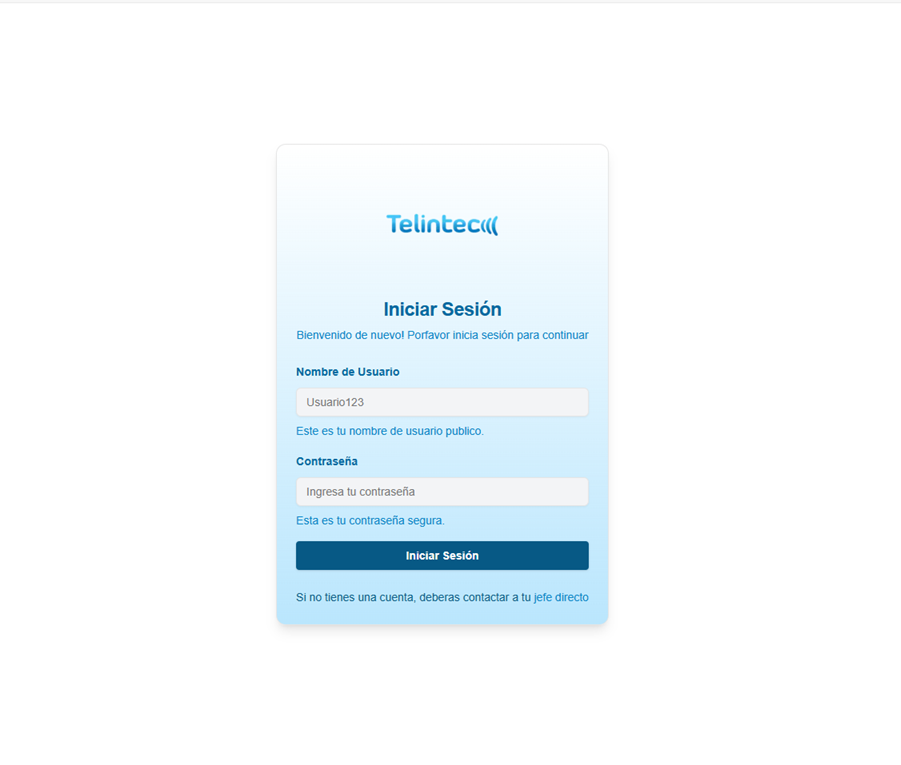
\includegraphics[width=0.6\textwidth]{imgs/inicio de sesion/inicio_sesion_desktop.png}
\caption{Ventana de inicio de sesión.}
\label{fig:login}
\end{figure}

\begin{justify}
A continuación, se describen los pasos para acceder a la plataforma, cómo proceder en caso de olvidar la contraseña y las recomendaciones de seguridad adaptadas a nuestro sistema. 
\end{justify}

\subsection{Acceso según rol de usuario}

\begin{itemize}
    \item  Departamento de Almacén: Los usuarios con este rol tendrán acceso exclusivo a las funcionalidades relacionadas con la gestión de inventarios, movimientos de productos, control de entradas y salidas, y generación de reportes y solicitud de materiales de almacén. 
    \item Departamento de Recursos Humanos: Los usuarios de este rol podrán utilizar las herramientas para la gestión de personal, control de asistencias, evaluación de desempeño, y otras funciones específicas del área de Recursos Humanos. 
\end{itemize}

Ventajas de este Modelo de Acceso:

\begin{itemize}
    \item Seguridad: Protege los datos sensibles asegurando que cada usuario acceda únicamente a la información y funcionalidades relevantes para su departamento. 
    \item Eficiencia: Facilita el uso del sistema al evitar distracciones con herramientas innecesarias para su rol. 
    \item Trazabilidad: Permite rastrear y auditar las acciones realizadas dentro del sistema según el rol del usuario. 
\end{itemize}

\subsection{Proceso de inicio de sesión}
\begin{enumerate}
    \item Ingreso de Credenciales 
    \item Accede a la página de inicio de sesión de Telintec a través de la URL proporcionada por el administrador de la empresa. 
    \item Introduce tu nombre de usuario y contraseña en los campos correspondientes. Estas credenciales serán proporcionadas por el administrador del sistema. 
    \item Haz clic en el botón "Iniciar sesión" para acceder a la plataforma. Si los datos son correctos, serás redirigido al panel principal de tu departamento (Almacén o Recursos Humanos). 
    \item Si no puedes acceder, verifica que tus credenciales sean correctas o consulta el procedimiento en caso de olvido de contraseña. 
\end{enumerate}

\subsection{Recuperación de Contraseña }
\begin{justify}

Actualmente, el sistema Telintec no dispone de una opción automatizada para recuperar contraseñas. En caso de que olvides tu contraseña: 
\end{justify}
\begin{enumerate}
    \item Contacta al equipo de soporte técnico de Telintec a través de los canales establecidos (correo electrónico o línea de soporte). 
    \item Proporciona tus datos de identificación, como nombre completo, correo registrado y departamento, para validar tu identidad. 
    \item El equipo técnico te asistirá en la generación de una nueva contraseña y en la actualización de tus credenciales de acceso. 
    \item Es importante mantener un registro seguro de tus credenciales para evitar interrupciones en el acceso al sistema. 
\end{enumerate}


\subsection{Recomendaciones de seguridad}
\begin{justify}
    Para proteger tu cuenta y los datos manejados por el sistema Telintec, sigue estas recomendaciones: 

\end{justify}

\begin{itemize}
    \item \textbf{Guarda tus credenciales en un lugar seguro:} Mantén un registro de tu usuario y contraseña en un lugar protegido, evitando compartir esta información.
    
    \item \textbf{Cambia tu contraseña regularmente:} Solicita al equipo de soporte que actualice tus credenciales periódicamente para fortalecer la seguridad.
    
    \item \textbf{Evita guardar tu contraseña en dispositivos compartidos:} Si utilizas una computadora o dispositivo no personal, asegúrate de no guardar la contraseña en el navegador.
    
    \item \textbf{Cierra sesión al terminar:} Siempre cierra sesión al finalizar tu uso del sistema, especialmente en dispositivos compartidos.
    
    \item \textbf{Reporta accesos no autorizados y utiliza conexiones seguras:} Si notas alguna actividad inusual o sospechosa en tu cuenta, notifícalo de inmediato al equipo de soporte técnico. Además, accede al sistema solo desde redes confiables para evitar posibles vulnerabilidades.
\end{itemize}

       


\chapter{Almacen}
\begin{justify}
    El Departamento de Almacén es una sección esencial dentro de la aplicación Telintec, diseñada para gestionar el inventario, registrar movimientos de productos y facilitar el control eficiente de materiales. A continuación, se describen las funciones de cada pestaña dentro de este departamento. 
\end{justify}
\begin{justify}
Estas pestañas permite la gestión detallada de los productos dentro del almacén. Las funcionalidades principales son: inventario, movimientos  y despacho de solicitudes de material
\end{justify}


\newpage
\pagestyle{fancy}

\section{Panel principal-\textit{Dashboard}}
\begin{justify}
    El Panel Principal del sistema Telintec es la interfaz inicial, mostrada en las figuras \ref{fig:dashboard}, que cada usuario ve después de iniciar sesión. Este panel está diseñado para adaptarse al rol y departamento del usuario, mostrando únicamente las funciones y herramientas autorizadas para su perfil. 
\end{justify}


\begin{figure}[ht!]
\centering
\begin{subfigure}{0.45\textwidth}
    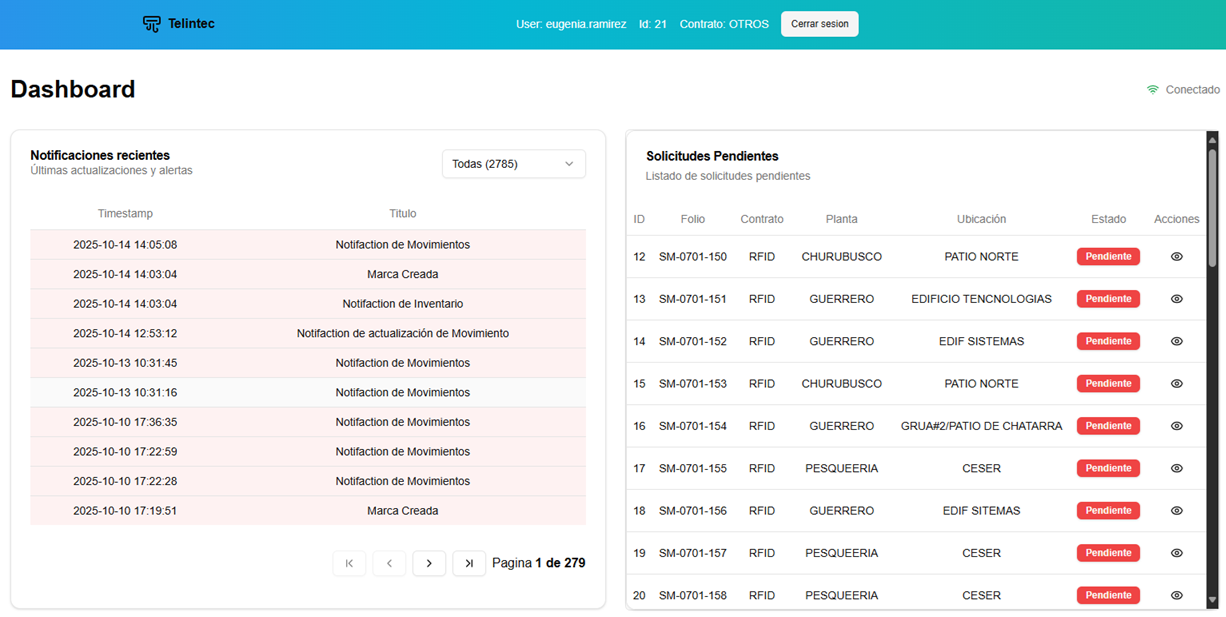
\includegraphics[width=\textwidth]{imgs/Almacen General/Dashboard/almacen_deahboard.png}
    \caption{Ventana de dashboard.}
    \label{fig:dash1}
\end{subfigure}
\hfill
\begin{subfigure}{0.45\textwidth}
    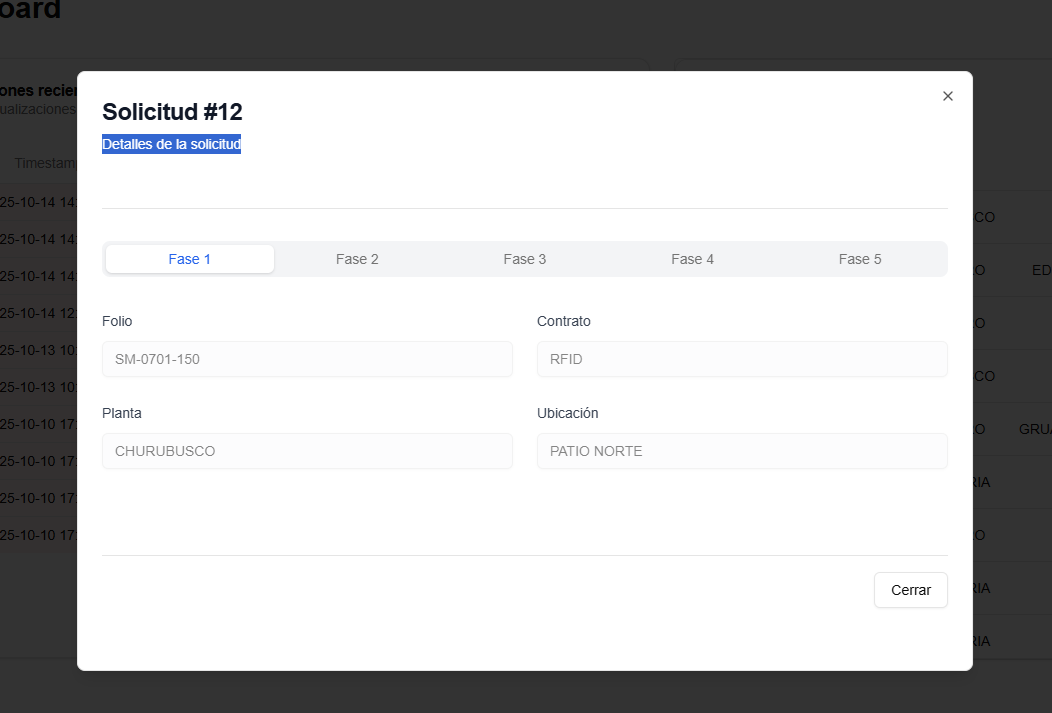
\includegraphics[width=\textwidth]{imgs/Almacen General/Dashboard/almacen_acciones.png}
    \caption{Acciones - Solicitudes pendientes.}
    \label{fig:dash2}
\end{subfigure}        
\caption{Panel de inicio.}
\label{fig:dashboard}
\end{figure}



\subsection{Características de la Pestaña Inicio} 

Una vez que el usuario inicia sesión, es redirigido automáticamente a su Dashboard, donde podrá visualizar: 
La pestaña "Inicio" del sistema Telintec ofrece diversas funcionalidades clave para el usuario:
\begin{itemize}
    \item \textbf{Notificaciones sobre el inventario:} En esta sección, podrás ver las notificaciones de las acciones realizadas en el inventario, como:
    \begin{itemize}
        \item \textbf{Creación de productos:} Se mostrará una notificación cuando se haya agregado un nuevo producto al inventario.
        \item \textbf{Eliminación de productos:} Aquí aparecerá una notificación si algún producto ha sido eliminado del inventario.
        \item \textbf{Actualización de productos:} Si algún producto ha sido actualizado (por ejemplo, cambios en la descripción, precio o cantidad), se mostrará una notificación indicando la acción realizada.
    \end{itemize}

    \item \textbf{Notificaciones de movimientos:} También se notifican los movimientos de productos dentro del sistema, tales como:
    \begin{itemize}
        \item \textbf{Entrada/Salida de productos:} Cuando los productos tengan salida y entrada, se registran en el inventario.
    \end{itemize}

    \item \textbf{Acciones destacadas:} Las acciones más importantes o urgentes aparecerán de manera destacada para que el usuario las identifique fácilmente.

    \item \textbf{Estadística:} En esta sección, se presentan datos clave sobre el estado y movimiento del inventario en forma de gráficos.
\end{itemize}

\subsubsection{Notificaciones relevantes}

En el caso de los empleados del departamento de Almacén, las notificaciones incluyen los diferentes estados de las Solicitudes de Material (SM), como solicitudes pendientes, en proceso o completadas. Estas notificaciones permiten a los usuarios mantenerse actualizados sobre las actividades clave de su área. 

\subsubsection{Menú principal personalizado}
El menú principal se adapta a las necesidades del usuario, presentando únicamente las opciones y pestañas autorizadas según su rol. Esto optimiza la experiencia del usuario y evita la confusión al eliminar elementos innecesarios. 

\subsection{Elementos comunes del dashboard }

El Dashboard incluye herramientas accesibles para todos los usuarios, como: 

\begin{itemize}
    \item Notificaciones: Indicadores visuales que alertan sobre acciones pendientes o eventos importantes relacionados con el departamento. 
    \item Menú Principal: Un acceso rápido a las principales pestañas y subpestañas relacionadas con las funciones del usuario. 
    \item Configuraciones: Opciones para actualizar el perfil del usuario, como el cambio de contraseña o ajustes de idioma. 
\end{itemize}


\subsection{Funcionalidades para almacén}

Para los empleados del almacén, el panel de inicio también incluye un acceso directo a las principales funciones operativas, organizadas en las siguientes pestañas: 

\begin{itemize}
    \item Inicio: Vista general de las notificaciones y acceso rápido a estados de Solicitudes de Material (SM). 
    \item Almacén: Inventario: Consulta y gestión de los productos disponibles en el almacén. 
    \item Movimientos: Registro y seguimiento de entradas y salidas de productos. 
    \item Procesamiento de SM: Herramienta para gestionar las solicitudes de material, desde su creación hasta su finalización. 
    \item Seguridad: Control y auditoría de accesos y actividades dentro del sistema. 
\end{itemize}

Este diseño modular asegura que cada usuario tenga acceso directo y simplificado a las funciones que necesita para cumplir sus tareas de manera eficiente y segura. 

 

\section{Inventario}
\begin{justify}
En esta pestaña, los usuarios pueden gestionar los productos en la base de datos, ya sea para dar de alta un nuevo producto, actualizar información existente o generar reportes.
\end{justify}
\begin{justify}
Registro de productos: Los usuarios pueden registrar nuevos productos en el sistema, incluyendo información clave como códigos, descripciones, categorías, proveedor y marca. La interfaz para estas operaciones se puede observar en las figuras \ref{fig:inventory}. Es importante resaltar que se puede agregar el código de barras manualmente. 
\end{justify}

\begin{figure}[ht!]
\centering
\begin{subfigure}{0.45\textwidth}
    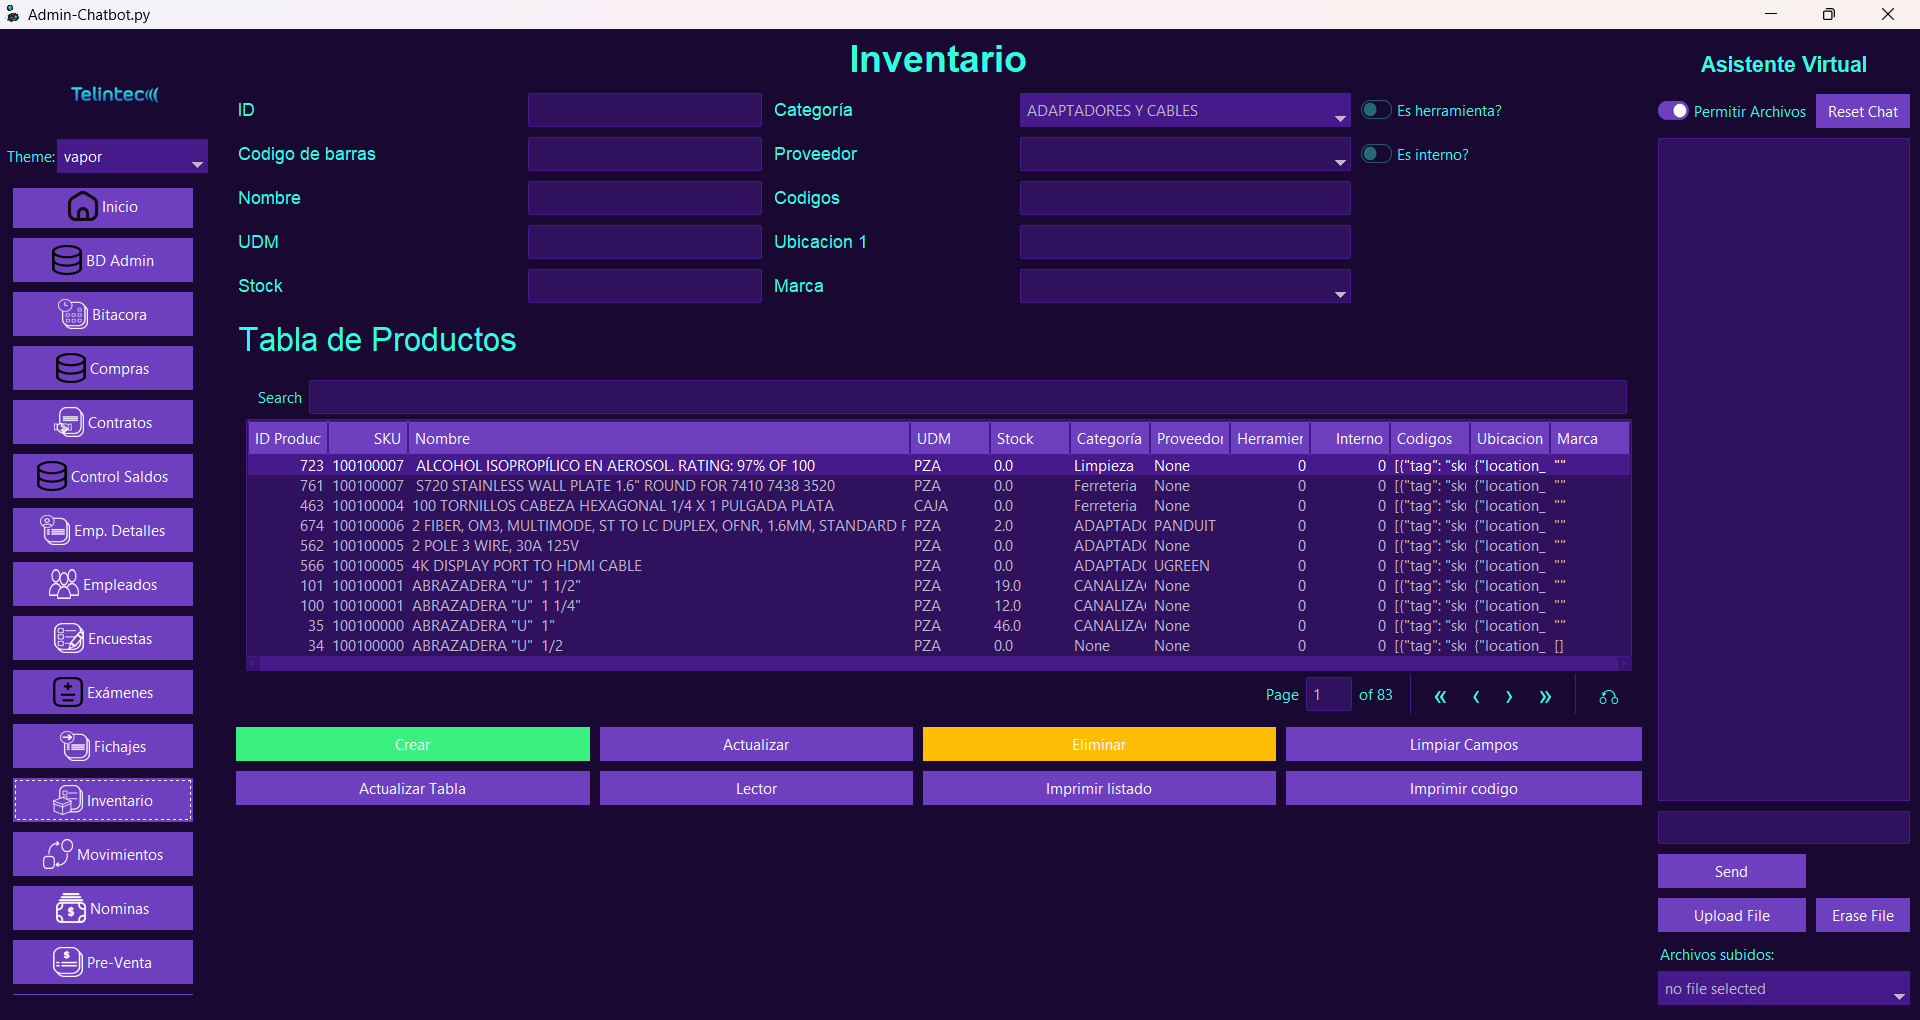
\includegraphics[width=\textwidth]{imgs/InventoryApp.png}
    \caption{Aplicación de escritorio.}
    \label{fig:invent1}
\end{subfigure}
\hfill
\begin{subfigure}{0.45\textwidth}
    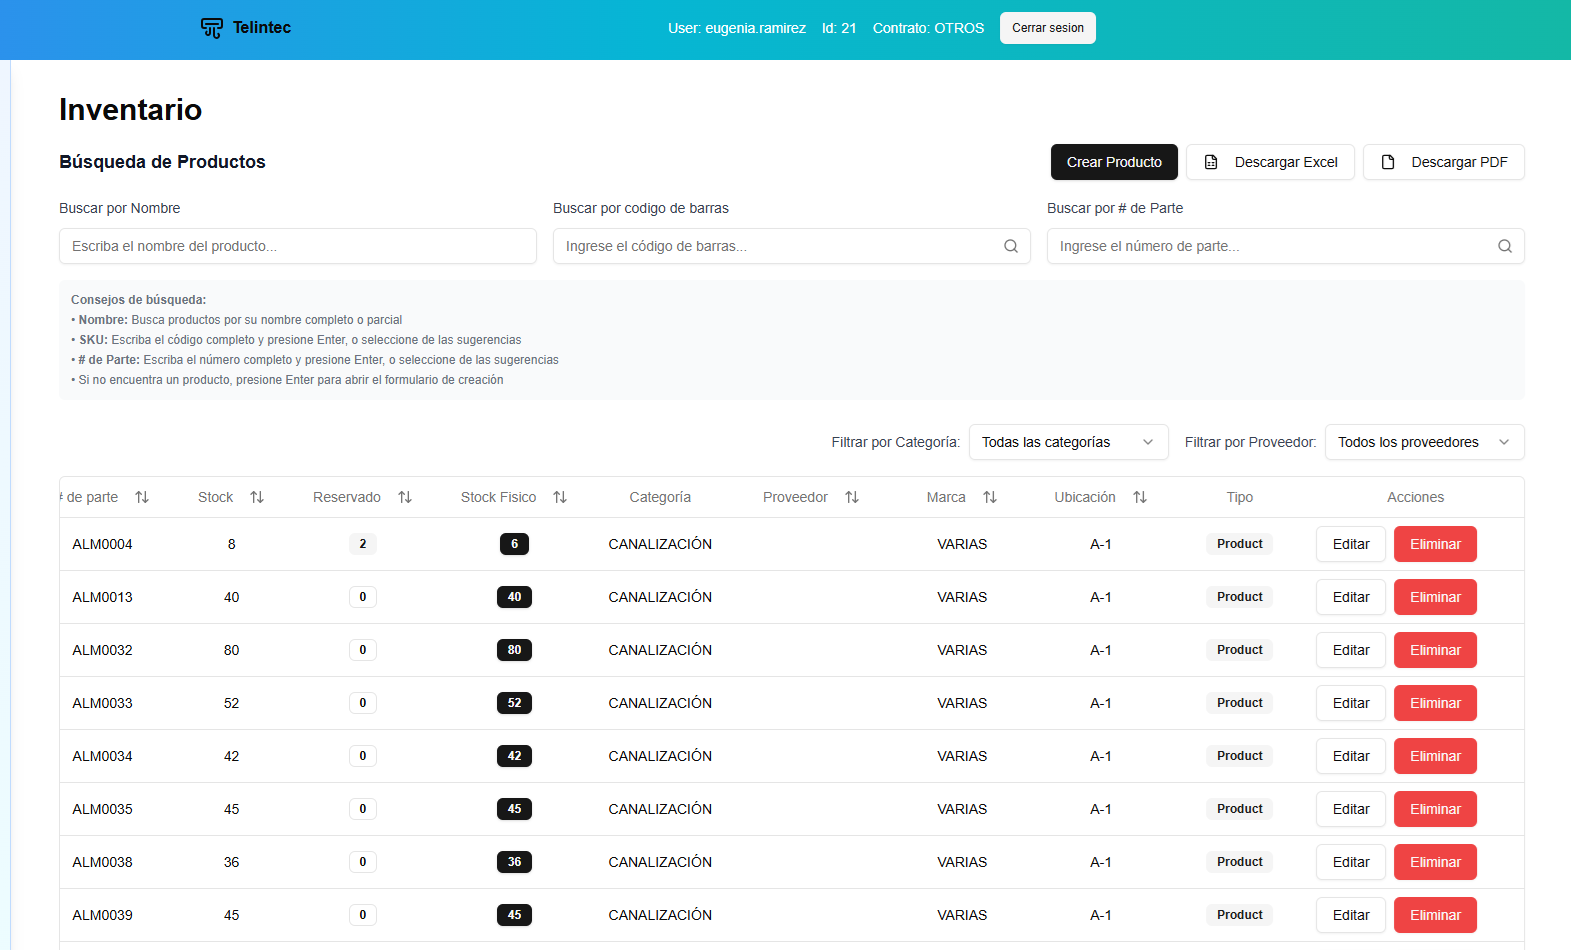
\includegraphics[width=\textwidth]{imgs/Almacen General/inventario/inventario_1_general.png}
    \caption{Apliación web.}
    \label{fig:invent2}
\end{subfigure}        
\caption{Ventana de inventario.}
\label{fig:inventory}
\end{figure}




Además, hay algunas restricciones del sistema que deben tomarse en cuenta: 

Al dar de alta un producto nuevo en el inventario, este puede registrarse mediante escáner o manualmente, y es obligatorio llenar todos los campos solicitados. Si se desea actualizar el stock de un producto existente, es necesario considerar que algunos productos antiguos pueden no tener información completa, como categoría, proveedor o códigos. Esto podría generar errores si no se actualizan estos campos junto con el stock. 

Es fundamental ser preciso al llenar el campo de “códigos”, ya que no se aceptan caracteres especiales. Funciones principales: La pestaña también permite realizar acciones clave como: 

\begin{itemize}
    \item Crear, actualizar y eliminar productos. 

    \item Actualizar la tabla donde se visualizan los productos. 

    \item Limpiar campos para facilitar el ingreso de nueva información. 

    \item Imprimir códigos, permitiendo crear y personalizar etiquetas de productos. 

    \item Utilizar el lector para escanear productos y registrar datos de manera rápida y precisa. 

    \item Consulta de existencias: Proporciona una vista actualizada de las existencias de productos disponibles, mostrando detalles como cantidades en almacén, ubicación y alertas de stock bajo. Además, el sistema permite visualizar los productos mediante una tabla, con la opción de buscarlos utilizando un buscador integrado. 
\end{itemize}

\section{Movimientos}

\subsection{Entradas}
Esta pestaña (Figura \ref{fig:ins}) se centra en la administración de los movimientos de inventario, ofreciendo las siguientes funciones: 

\begin{figure}[ht!]
\centering
\begin{subfigure}{0.45\textwidth}
    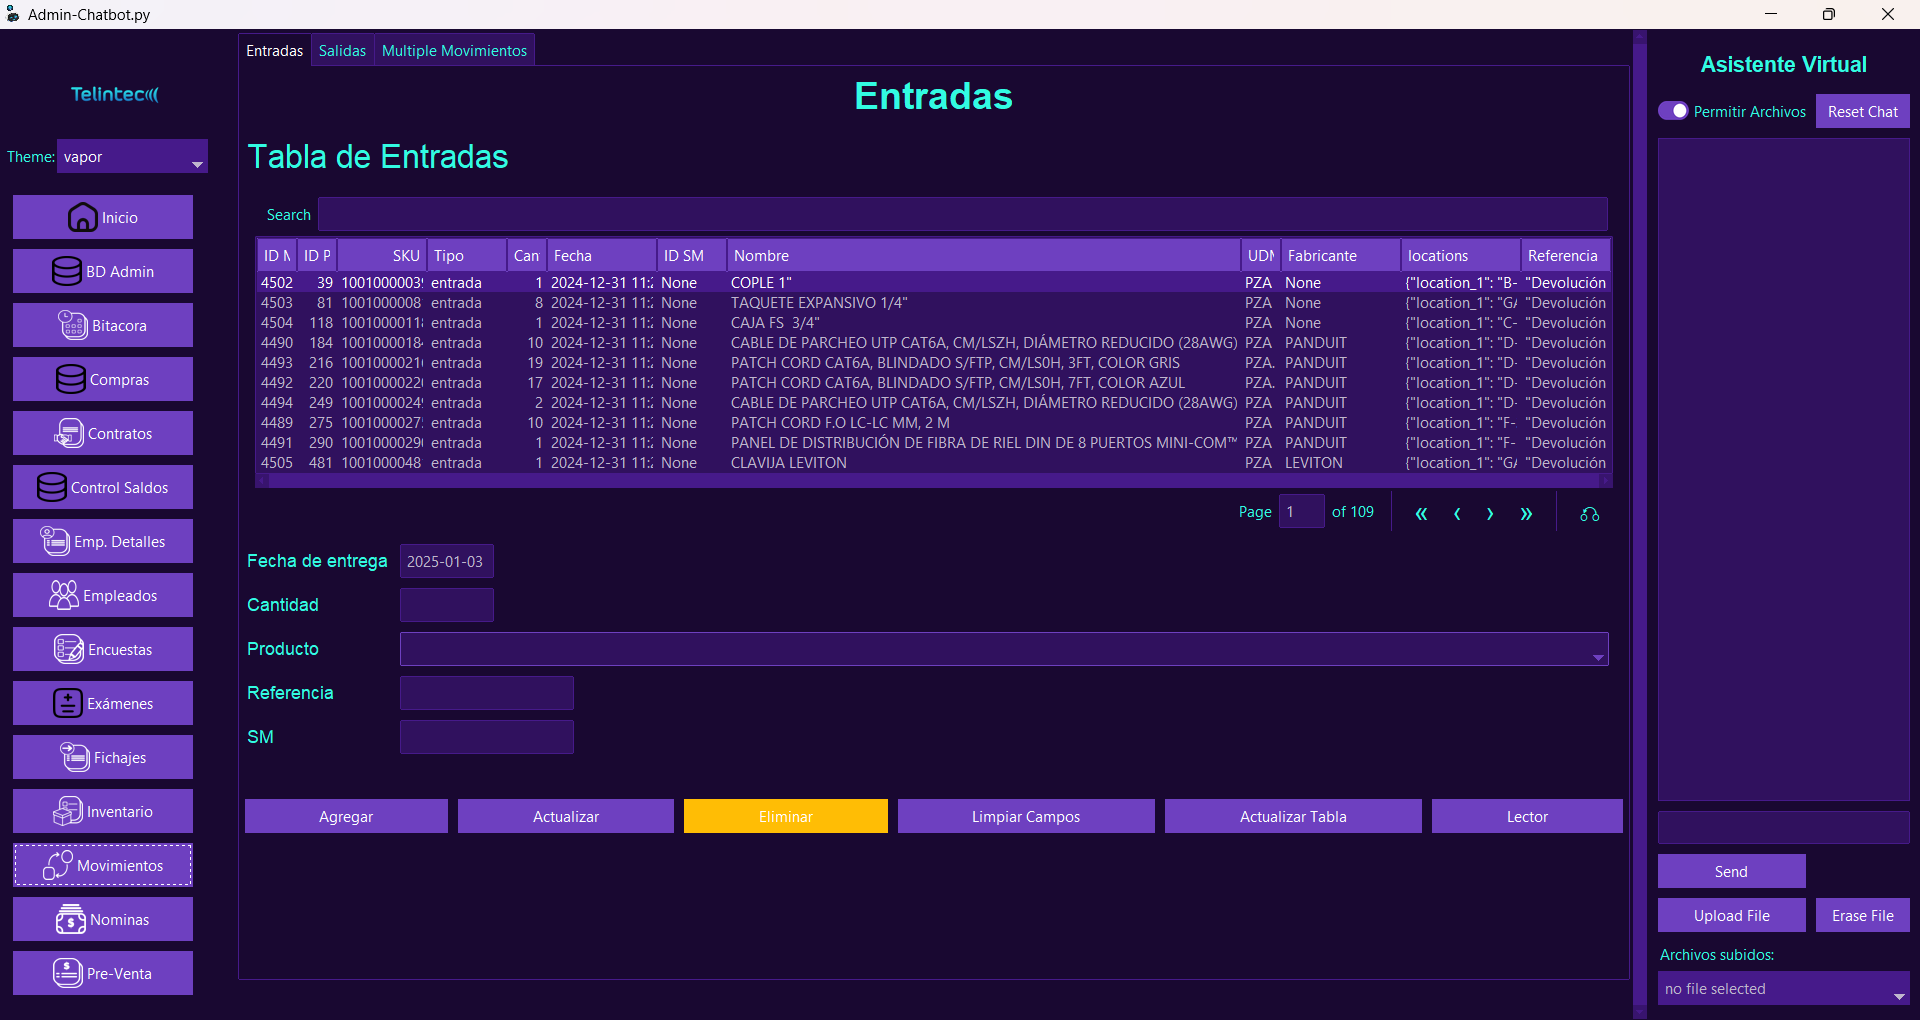
\includegraphics[width=\textwidth]{imgs/InsApp.png}
    \caption{Aplicación de escritorio.}
    \label{fig:ins1}
\end{subfigure}
\hfill
\begin{subfigure}{0.45\textwidth}
    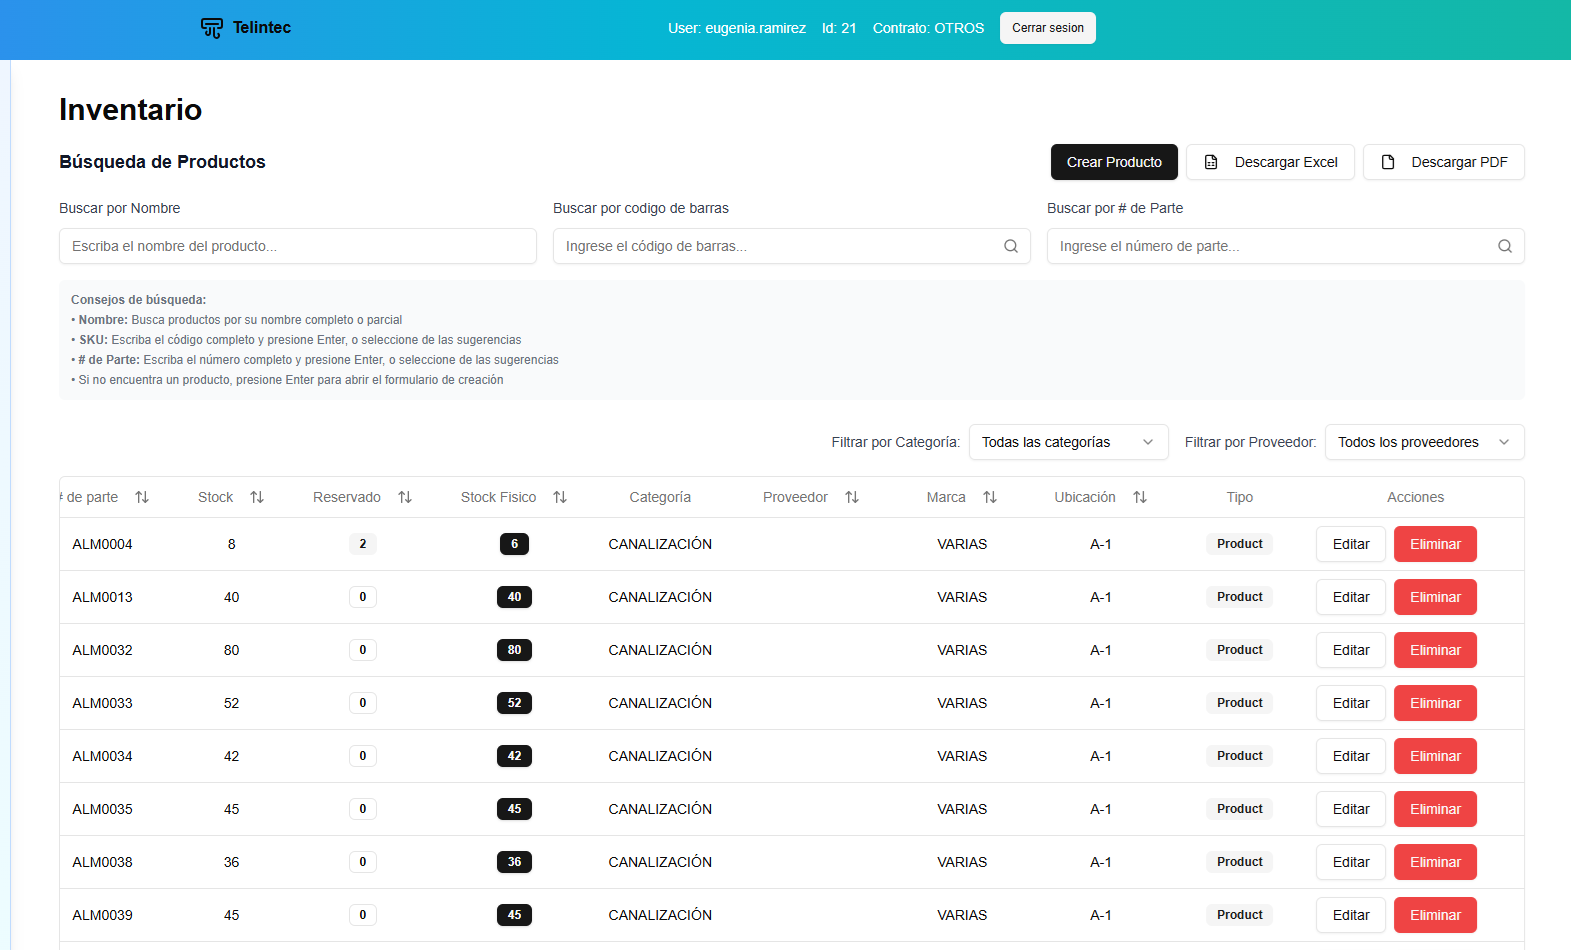
\includegraphics[width=\textwidth]{imgs/Almacen General/inventario/inventario_1_general.png}
    \caption{Apliación web.}
    \label{fig:ins2}
\end{subfigure}        
\caption{Ventana de creación de entradas.}
\label{fig:ins}
\end{figure}



Aquí, se permite registrar la recepción de productos en el inventario, ya sea por compras, devoluciones o ajustes. Visualiza los productos y ofrece las opciones de agregar una nueva entrada, actualizarla o eliminarla. Incluye un lector de código de barras para escanear los productos existentes a los cuales se desea dar entrada. 
\textbf{Importante}: No es posible crear productos directamente desde esta opción de entrada. 

\subsection{Salidas}

En esta interfaz (Figura \ref{fig:outs}), se facilita el registro de productos que salen del almacén, ya sea por ventas o devoluciones de clientes. Puedes crear, actualizar o eliminar una salida, y también hacerlo utilizando el lector de código de barras, simplemente escaneando el producto y completando los campos requeridos. 

\begin{figure}[ht!]
\centering
\begin{subfigure}{0.45\textwidth}
    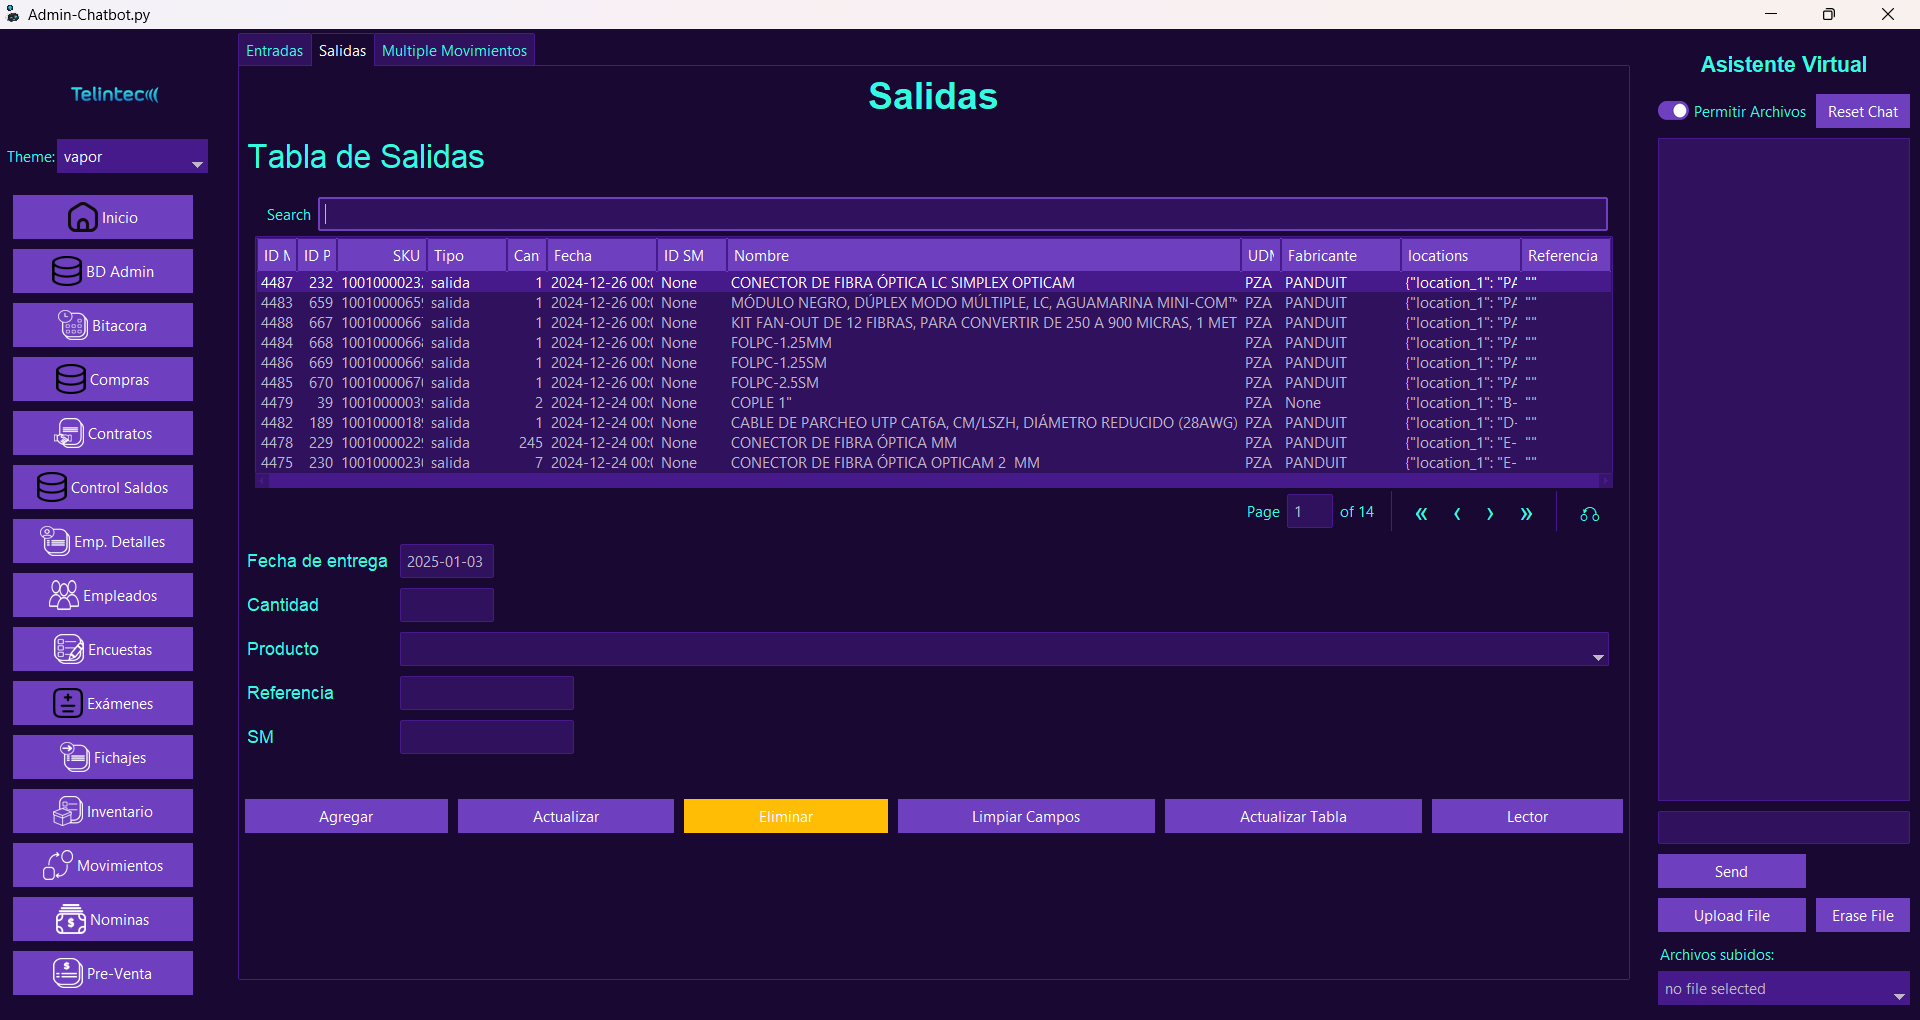
\includegraphics[width=\textwidth]{imgs/OutsApp.png}
    \caption{Aplicación de escritorio.}
    \label{fig:outs1}
\end{subfigure}
\hfill
\begin{subfigure}{0.45\textwidth}
    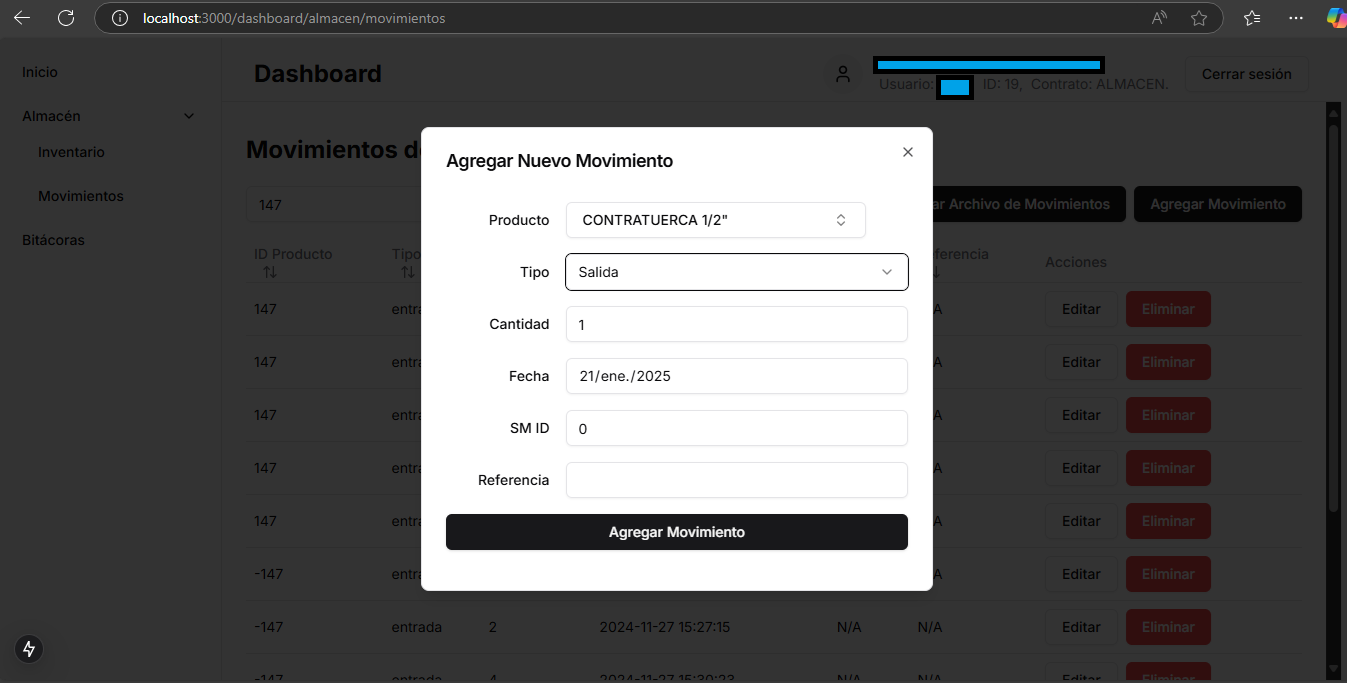
\includegraphics[width=\textwidth]{imgs/OutsWebApp.png}
    \caption{Apliación web.}
    \label{fig:outs2}
\end{subfigure}        
\caption{Ventana de inventario.}
\label{fig:outs}
\end{figure}

\textbf{Consideración}: Algunos productos más antiguos en el sistema tienen restricciones al intentar actualizar el stock. Si es necesario, deberás actualizar también nuevos campos que se añadan a petición de administración. 

\subsection{Movimientos múltiples} 
\begin{figure}[ht!]
\centering
\begin{subfigure}{0.45\textwidth}
    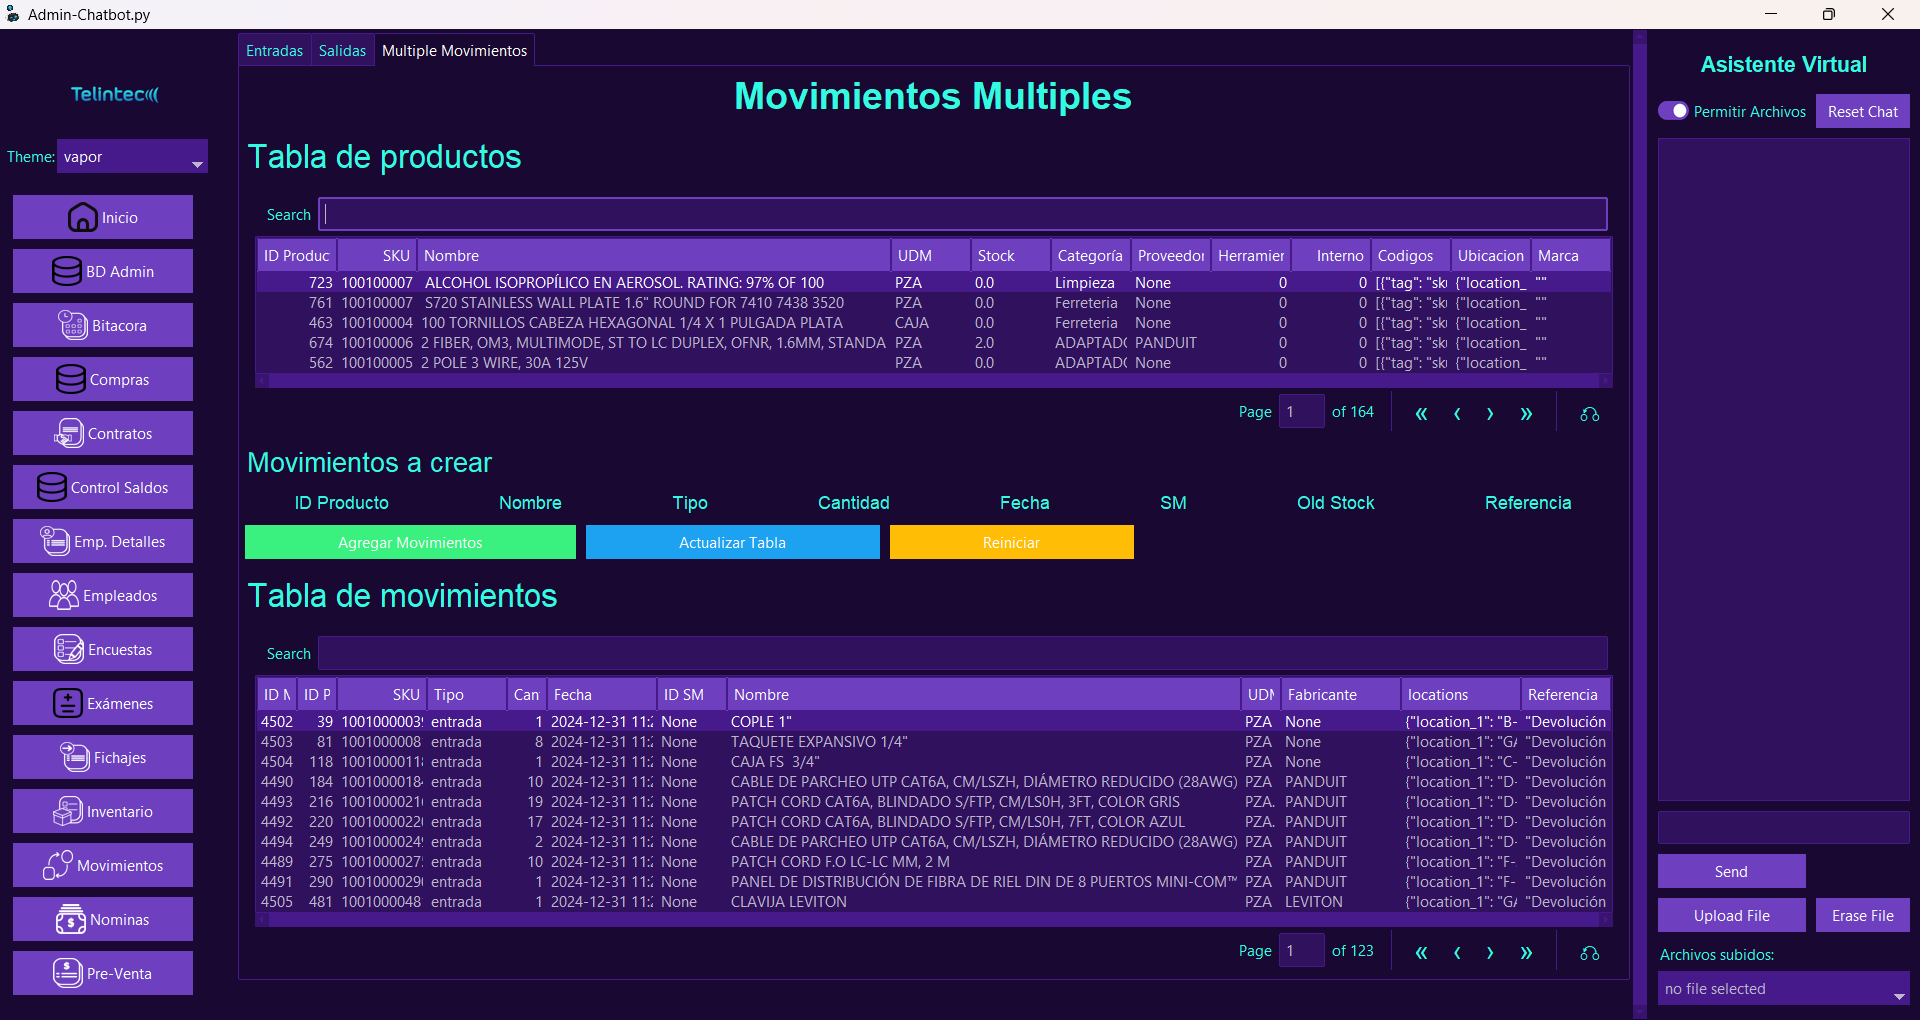
\includegraphics[width=\textwidth]{imgs/MultipleMovesApp.png}
    \caption{Aplicación de escritorio.}
    \label{fig:multimoves1}
\end{subfigure}
\hfill
\begin{subfigure}{0.45\textwidth}
    
\includegraphics[width=0.5\textwidth]{imgs/no-image.png}
    \caption{Apliación web.}
    \label{fig:multimoves2}
\end{subfigure}        
\caption{Ventana de ingreso de multiples movimientos.}
\label{fig:multimoves}
\end{figure}

Esta  interfaz (Figura \ref{fig:multimoves}) opción permite crear entradas y salidas simultáneamente para varios productos, los cuales se agregarán en forma de lista. El campo \textit{Old Stock} es solo una etiqueta visual para que puedas ver el stock actual. \textbf{No deberás modificar este campo.} 

\section{Solicitudes de Material}

Esta pestaña está diseñada para facilitar el proceso de solicitud y aprobación de materiales dentro de la organización. Sus funcionalidades incluyen: 

Creación de solicitudes: Permite a los usuarios generar solicitudes de material de manera rápida, especificando detalles como cantidades requeridas, razones de uso y fechas necesarias. 

Aprobación y seguimiento: Los administradores pueden aprobar o rechazar solicitudes y realizar un seguimiento de su estado hasta la entrega final. 

\section{Escaner}

La pestaña del escáner está enfocada en optimizar el registro de movimientos de inventario mediante el uso de tecnología de códigos de barras. Para la aplicación de escritorio se despliega una ventana extra donde se realizan las operaciones del lector. Las funciones disponibles son: 

\begin{figure}[ht!]
\centering
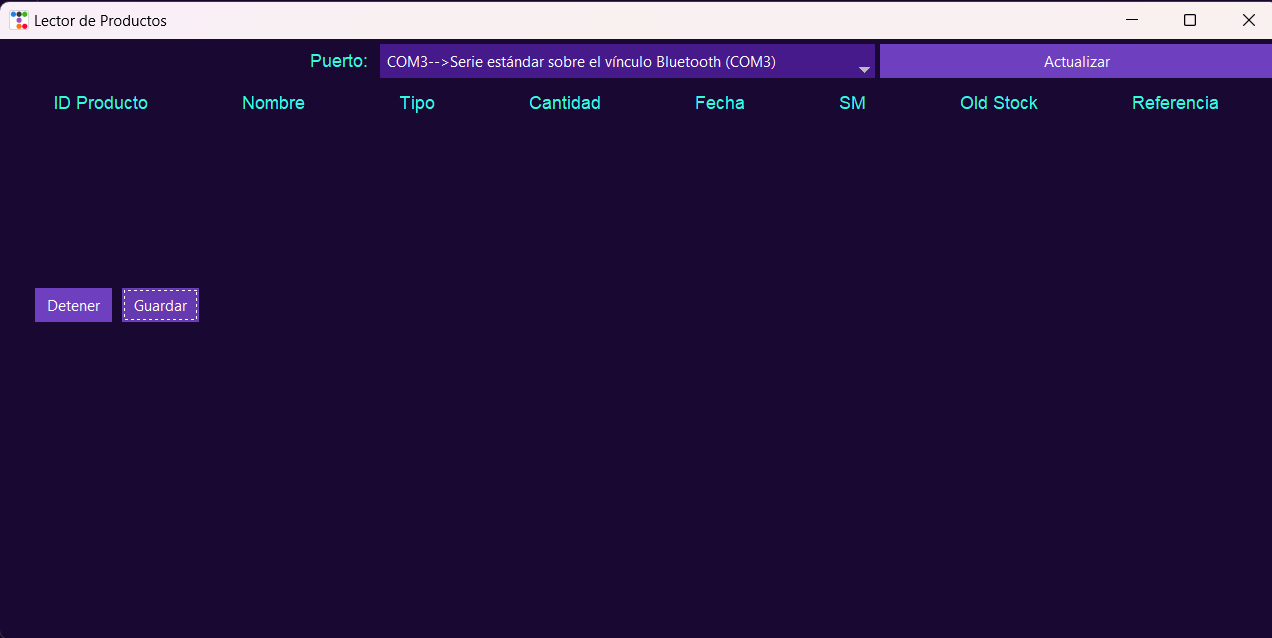
\includegraphics[width=0.7\textwidth]{imgs/LectorApp.png}
\caption{Ventana emergente para funcines del lector.}
\label{fig:lecotr}
\end{figure}

Permite a los usuarios registrar entradas y salidas de manera rápida y precisa escaneando los códigos de barras de los productos. Esto facilita la gestión del inventario de manera eficiente y sin errores manuales.

\textbf{¿El escáner se desconfiguró?} Sigue estos pasos:
\begin{enumerate}
    \item Verifica la conexión: Asegúrate de que el escáner esté correctamente conectado al dispositivo. Si es inalámbrico, comprueba que esté dentro del rango de la red o que la batería esté cargada. 

    \item Reinicia el escáner: Apaga el escáner y vuélvelo a encender para restablecer su configuración. 

    \item Reconfigura el escáner: 
    \begin{itemize}
        \item Escanea el código de configuración que aparece en el manual del escáner para restablecer los ajustes predeterminados.
        \item Puedes acceder al manual desde el 
        \href{https://drive.google.com/file/d/1OsTJD1-Hbvdd9wIGknSJqKVfENMQDajR/view?usp=sharing.}{\emph{enlace}}. 
        \item Este manual incluye los códigos necesarios y las instrucciones detalladas para la configuración.
    \end{itemize}
    \item Verifica la configuración del software. Asegúrate de buscar en tu dispositivo el administrador de dispositivos los puertos (COM) y poder ver si el escáner ya es reconocido por el dispositivo.

    \item Consulta la guía de solución de problemas. Si el escáner sigue sin funcionar correctamente, consulta la guía de solución de problemas para verificar posibles errores de lectura o ajustes necesarios. 
\end{enumerate}
\chapter{Administración }


Este módulo permite gestionar la base de datos de clientes y proveedores, contratos, órdenes de compra y entregas de solicitudes de material.
\newpage
\pagestyle{fancy}

\subsection{3.1 Base de datos}

\subsubsection{3.1.1 Gestión de Base de Datos – Pestaña: Clientes}

En esta pestaña puedes:

\begin{itemize}
    \item Registrar nuevos clientes.
    \item Editar información existente.
    \item Buscar clientes por nombre o ID.
\end{itemize}

\begin{figure}[h]
\centering
\begin{subfigure}{0.4\textwidth}
    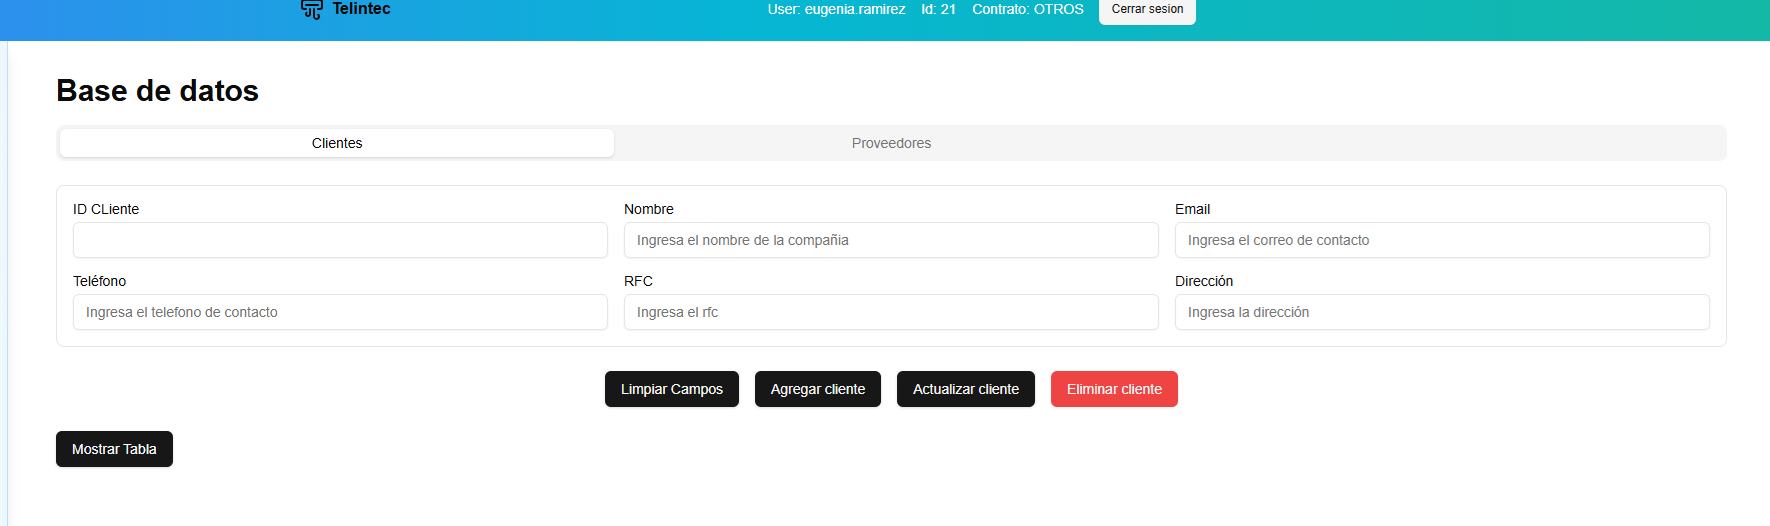
\includegraphics[width=\textwidth]{imgs/Administracion/BASE DE DATOS/administracion-BASEDEDATOS/ad_bd_provedores_tabla.png}
    \caption{Gestión de clientes.}
    \label{fig:admin1}
\end{subfigure}
\caption{Interfaz de clientes en la base de datos.}
\end{figure}

\subsubsection{3.1.2 Gestión de Base de Datos – Pestaña: Proveedores}

Funciones disponibles:

\begin{itemize}
    \item Alta de proveedores.
    \item Edición de datos como razón social, RFC, contacto.
    \item Filtro por tipo de proveedor.
\end{itemize}

\begin{figure}[h]
\centering
\begin{subfigure}{0.4\textwidth}
    
\includegraphics[width=\textwidth]{imgs/no-image.png}
    \caption{Gestión de proveedores.}
    \label{fig:admin2}
\end{subfigure}
\caption{Interfaz de proveedores en la base de datos.}
\end{figure}

\subsection{3.2 Contratos}

\subsubsection{3.2.1 Crear Contrato}

Para registrar un nuevo contrato:

\begin{itemize}
    \item Ingresa nombre del cliente, número de contrato, fecha de inicio y fin.
    \item Asocia el contrato a un proyecto si aplica.
    \item Guarda el contrato para que esté disponible en otras secciones del sistema.
\end{itemize}

\begin{figure}[h]
\centering
\begin{subfigure}{0.4\textwidth}
    
\includegraphics[width=\textwidth]{imgs/no-image.png}
    \caption{Formulario de contrato.}
    \label{fig:admin3}
\end{subfigure}
\caption{Creación de contrato en el sistema.}
\end{figure}

\subsubsection{Editar contrato}

Para modificar un contrato existente:

\begin{itemize}
    \item Usa el buscador para localizar el contrato.
    \item Haz clic en “Editar”.
    \item Actualiza los campos necesarios y guarda los cambios.
\end{itemize}

\subsection{3.3 Órdenes de compra}

\subsubsection{3.3.1 Crear orden de compra desde solicitud de material (SM)}

Desde una SM aprobada:

\begin{itemize}
    \item Selecciona los productos requeridos.
    \item El sistema autocompleta los datos del proveedor y contrato.
    \item Genera la orden de compra con folio único.
\end{itemize}

\begin{figure}[h]
\centering
\begin{subfigure}{0.4\textwidth}
    
\includegraphics[width=\textwidth]{imgs/no-image.png}
    \caption{Orden desde SM.}
    \label{fig:admin4}
\end{subfigure}
\caption{Creación de orden de compra desde solicitud de material.}
\end{figure}

\subsubsection{Crear Nueva orden de compra (manual)}

También puedes crear órdenes manualmente:

\begin{itemize}
    \item Ingresa proveedor, productos, cantidades y precios.
    \item Asocia la orden a un contrato si aplica.
    \item Guarda y descarga en PDF o Excel.
\end{itemize}

\subsection{3.4 Entregas de Solicitudes de material (SM)}

\subsubsection{3.4.1 Paso 1: Seleccionar una solicitud de material (SM)}

Para entregar materiales:

\begin{itemize}
    \item Selecciona una SM pendiente.
    \item Verifica productos disponibles y faltantes.
    \item Despacha los productos desde el almacén.
\end{itemize}

\begin{figure}[h]
\centering
\begin{subfigure}{0.4\textwidth}
    
\includegraphics[width=\textwidth]{imgs/no-image.png}
    \caption{Entrega de SM.}
    \label{fig:admin5}
\end{subfigure}
\caption{Interfaz de entrega de solicitudes de material.}
\end{figure}

\chapter{Almacén de Productos de Seguridad (EPP)}

Este módulo está diseñado para gestionar el inventario y la aprobación de vales relacionados con equipos de protección personal (EPP). Su objetivo es asegurar que los productos de seguridad estén disponibles, correctamente registrados y entregados conforme a los protocolos establecidos.

\subsection{Inventario de productos de Seguridad (EPP)}

En esta sección, los usuarios pueden consultar y administrar los productos de seguridad disponibles en el almacén.

\begin{itemize}
    \item Visualización de productos por categoría (guantes, cascos, chalecos, etc.).
    \item Registro de nuevos productos de seguridad.
    \item Edición de información como marca, proveedor y stock.
    \item Filtros por tipo de producto y proveedor.
\end{itemize}

\begin{figure}[h]
\centering
\begin{subfigure}{0.4\textwidth}
    
\includegraphics[width=\textwidth]{imgs/no-image.png}
    \caption{Inventario de EPP.}
    \label{fig:epp1}
\end{subfigure}
\caption{Vista del inventario de productos de seguridad.}
\end{figure}

\subsection{Aprobar Vales de Seguridad}

Esta función permite validar y autorizar la entrega de productos de seguridad solicitados por los colaboradores.

\begin{itemize}
    \item Revisión de solicitudes pendientes.
    \item Verificación de disponibilidad en inventario.
    \item Aprobación o rechazo de vales según criterios operativos.
    \item Registro automático del movimiento en el sistema.
\end{itemize}

\begin{figure}[h]
\centering
\begin{subfigure}{0.4\textwidth}
    
\includegraphics[width=\textwidth]{imgs/no-image.png}
    \caption{Aprobación de vales.}
    \label{fig:epp2}
\end{subfigure}
\caption{Interfaz para aprobar vales de seguridad.}
\end{figure}

\subsection{Flujo operativo de aprobación de vales}

El proceso de aprobación sigue un flujo estructurado:

\begin{enumerate}
    \item El usuario solicita un vale de seguridad desde el módulo correspondiente.
    \item El sistema verifica el stock disponible.
    \item El responsable revisa la solicitud y aprueba o rechaza.
    \item Si se aprueba, el producto se despacha y se registra el movimiento.
    \item El vale queda marcado como completado en el sistema.
\end{enumerate}

\begin{figure}[h]
\centering
\begin{subfigure}{0.4\textwidth}
    
\includegraphics[width=\textwidth]{imgs/no-image.png}
    \caption{Flujo de aprobación.}
    \label{fig:epp3}
\end{subfigure}
\caption{Proceso operativo para vales de seguridad.}
\end{figure}
\chapter{Cargos}

Este módulo permite gestionar los cargos asignados a líderes, gerentes y otros colaboradores dentro de la organización. Su objetivo es mantener una estructura clara de responsabilidades y facilitar la trazabilidad de acciones en el sistema.

\subsection{Asignación de cargos}

La asignación de cargos se realiza desde una interfaz que permite:

\begin{itemize}
    \item Registrar nuevos cargos para usuarios existentes.
    \item Visualizar la lista de líderes y gerentes con sus cargos actuales.
    \item Editar cargos asignados previamente.
\end{itemize}

\begin{figure}[h]
\centering
\begin{subfigure}{0.4\textwidth}
    
\includegraphics[width=\textwidth]{imgs/no-image.png}
    \caption{Asignación de cargos.}
    \label{fig:cargos1}
\end{subfigure}
\caption{Interfaz para asignar cargos a colaboradores.}
\end{figure}

\subsection{Lista de líderes y gerentes con sus cargos}

La pantalla muestra una tabla con los siguientes campos:

\begin{itemize}
    \item Nombre del colaborador.
    \item Cargo asignado.
    \item Departamento.
    \item Fecha de asignación.
\end{itemize}

Esta lista permite filtrar por departamento o buscar por nombre para facilitar la gestión.

\begin{figure}[h]
\centering
\begin{subfigure}{0.4\textwidth}
    
\includegraphics[width=\textwidth]{imgs/no-image.png}
    \caption{Lista de cargos.}
    \label{fig:cargos2}
\end{subfigure}
\caption{Visualización de líderes y gerentes con sus cargos.}
\end{figure}

\subsection{Editar cargo}

Para modificar un cargo:

\begin{itemize}
    \item Selecciona al colaborador desde la lista.
    \item Haz clic en el botón “Editar”.
    \item Actualiza el cargo y guarda los cambios.
\end{itemize}

El sistema registrará la modificación y actualizará la trazabilidad del usuario.

\begin{figure}[h]
\centering
\begin{subfigure}{0.4\textwidth}
    
\includegraphics[width=\textwidth]{imgs/no-image.png}
    \caption{Edición de cargo.}
    \label{fig:cargos3}
\end{subfigure}
\caption{Formulario para editar cargos asignados.}
\end{figure}
\chapter{Operaciones}

Este módulo permite gestionar los vales de seguridad y herramientas/equipo, facilitando su creación, edición y trazabilidad. Está diseñado para que los responsables de almacén y operaciones puedan administrar entregas de forma eficiente.

\subsection{Vales}

\subsubsection{Ventana General de Vales}

La ventana principal muestra todos los vales registrados en el sistema, con filtros por tipo, estado y fecha.

\begin{itemize}
    \item Visualización de vales activos, completados o pendientes.
    \item Filtros por tipo de vale: seguridad o herramientas/equipo.
    \item Acciones disponibles: editar, imprimir, exportar.
\end{itemize}

\begin{figure}[h]
\centering
\begin{subfigure}{0.4\textwidth}
    
\includegraphics[width=\textwidth]{imgs/no-image.png}
    \caption{Vista general de vales.}
    \label{fig:operaciones1}
\end{subfigure}
\caption{Panel principal del módulo de vales.}
\end{figure}

\subsubsection{Crear vale de seguridad}

Para crear un vale de seguridad:

\begin{itemize}
    \item Selecciona el colaborador y el contrato asociado.
    \item Añade los productos de seguridad requeridos desde el catálogo.
    \item Verifica el stock disponible.
    \item Guarda el vale para que sea procesado por el área correspondiente.
\end{itemize}

\begin{figure}[h]
\centering
\begin{subfigure}{0.4\textwidth}
    
\includegraphics[width=\textwidth]{imgs/no-image.png}
    \caption{Creación de vale de seguridad.}
    \label{fig:operaciones2}
\end{subfigure}
\caption{Formulario para registrar un vale de seguridad.}
\end{figure}

\subsubsection{Editar vale de seguridad}

Para modificar un vale existente:

\begin{itemize}
    \item Localiza el vale en la lista general.
    \item Haz clic en “Editar”.
    \item Actualiza productos, cantidades o datos del colaborador.
    \item Guarda los cambios para actualizar el registro.
\end{itemize}

\begin{figure}[h]
\centering
\begin{subfigure}{0.4\textwidth}
    
\includegraphics[width=\textwidth]{imgs/no-image.png}
    \caption{Edición de vale de seguridad.}
    \label{fig:operaciones3}
\end{subfigure}
\caption{Interfaz para editar vales de seguridad.}
\end{figure}

\subsubsection{Crear vale de Herramientas/Equipo}

Este tipo de vale permite registrar la entrega de herramientas o equipos específicos.

\begin{itemize}
    \item Selecciona el tipo de herramienta o equipo.
    \item Asocia el vale a un contrato y colaborador.
    \item Verifica disponibilidad y guarda el registro.
\end{itemize}

\begin{figure}[h]
\centering
\begin{subfigure}{0.4\textwidth}
    
\includegraphics[width=\textwidth]{imgs/no-image.png}
    \caption{Vale de herramientas/equipo.}
    \label{fig:operaciones4}
\end{subfigure}
\caption{Formulario para crear vales de herramientas.}
\end{figure}

\subsubsection{Editar vale de Herramientas/Equipo}

Para modificar un vale de herramientas:s

\begin{itemize}
    \item Accede a la lista de vales.
    \item Selecciona el vale a editar.
    \item Cambia productos, cantidades o datos del responsable.
    \item Guarda los cambios.
\end{itemize}

\begin{figure}[h]
\centering
\begin{subfigure}{0.4\textwidth}
    
\includegraphics[width=\textwidth]{imgs/no-image.png}
    \caption{Edición de vale de herramientas.}
    \label{fig:operaciones5}
\end{subfigure}
\caption{Interfaz para editar vales de herramientas/equipo.}
\end{figure}
\chapter{Principales Procesos}

Este módulo describe el flujo de validación de vales dentro del sistema Telintec, asegurando que cada entrega de productos esté correctamente registrada, aprobada y trazada. Es clave para mantener la integridad operativa entre almacén, administración y operaciones.

\subsection{Flujo de validación de vales}

El proceso de validación de vales sigue una secuencia estructurada que involucra distintos roles y etapas:

\begin{enumerate}
    \item \textbf{Creación del vale:} El usuario solicita un vale desde el módulo correspondiente, seleccionando productos, cantidades y contrato asociado.
    \item \textbf{Verificación de stock:} El sistema revisa la disponibilidad de los productos en el inventario.
    \item \textbf{Aprobación del vale:} El responsable del área revisa la solicitud y aprueba o rechaza según criterios operativos.
    \item \textbf{Despacho de productos:} Una vez aprobado, el almacén realiza la entrega física del producto.
    \item \textbf{Registro del movimiento:} El sistema actualiza el inventario y marca el vale como completado.
\end{enumerate}

\begin{figure}[h]
\centering
\begin{subfigure}{0.4\textwidth}
    
\includegraphics[width=\textwidth]{imgs/no-image.png}
    \caption{Flujo de validación.}
    \label{fig:procesos1}
\end{subfigure}
\caption{Proceso completo de validación de vales en Telintec.}
\end{figure}

Este flujo garantiza trazabilidad, control y eficiencia en la entrega de materiales, alineando las acciones del sistema con los procesos internos de la empresa.

\end{document}
